\chapter{Related Work}\label{sec:related-work}
Hauder et al. mention numerous research challenges in the domain of ACM, among them an active support system for knowledge workers \cite{hauder2014}.
The need for such a system is emphasized by Francescomarino et al. in their literature review, where it has been found that few prediction approaches target the next activity \cite{francescomarino2018}.\\

With the focus of this thesis put on improving next activity predictions, the domains of process science and data science are brought together. In both, research has been published on sequence prediction. In the former in the context of processes and events and the latter in the context of natural language. By topic, the related works in these domains shall be presented in this chapter.
\todo[inline]{Furthermore they may be some research on Neural Network Architecture?!}

\section{Process prediction}
\marginpar{CoCaMa is an abbreviation for a project called Collaborative Case Management, which appears to be retired: \href{http://archive.li/uZFnN}{archive.li/uZFnN}}
An example for how such a support system \cite{hauder2014} might look like is given by Huber, who has developed a next-step prediction and recommendation system. The system is prototypically implemented within CoCaMa, a case management application.

After gathering the training data from various sources via an extract, transform and load (ETL) process, several \textit{Next Models} are constructed. The Next Models are a collection of predictive models used to predict the next activity, focused on different criteria: remaining time, constraint violation, decisions based on case-specific data, and case outcome. The weighting of the predictions from these individual models is non-trivial and extensively discussed. Huber models the prediction as a classification problem and uses decision trees from the WEKA \cite{web:weka} machine learning toolkit to implement them. The system has been evaluated with 25 hand-made case logs \cite{huber2015}.\\

Building upon each other are the works by Evermann et al. \cite{evermann2016} and Schönig et al. \cite{schoenig2018}. Evermann et al. remark the lack of research on next event predictions and have successfully demonstrated the applicability of LSTM neural networks in the context of predicting the next activity. Using a neural network implemented with Tensorflow, precision in excess of $90\%$ on the BPIC2012 and BPIC2013 datasets was achieved. Evermann et al. want their work to be understood as a "demonstration of the applicability of the approach and the potential for future work". The authors highlight the lacking use of data attributes during model training as well as the fact that the count of LSTM cells was not set in relation to trace length.

Schönig et al. \cite{schoenig2018} picked up on Evermann's related work and demonstrated on BPIC datasets from 2017 that using data attributes does increase prediction accuracy. Schönig et al. implemented their solution with Keras and trained it using stratified 5-fold cross-validation. The data was formatted with the sliding window method of width 1. The work nicely demonstrates that an increasing number of included data attributes can continually improve accuracy \cite[p.5]{schoenig2018}

Similar to Schönig et al., Polato et al. make use of data attributes in their work for improving the prediction of the remaining time of business process instances \cite{polato2014}. During feature engineering, their SVR training data is enriched with information about possible other activities. Unfortunately, Polato et al. do not list which dataset they have used\\
\todo[inline]{Verify whether they actually do not mention it}

Metzger et al. predict run-time of a case by comparing and combining different prediction models into a model ensemble. Then, the members of the ensemble are selected based on their predictive performance measures. This allows taking into account costs of false predictions \cite{metzger2015}.\\

Francescomarino et al. have performed clustering in the preprocessing phase of model training and prediction. Having clustered the training data, one model was created and trained for each cluster. For obtaining a prediction, the cluster for a new data item is found from which the corresponding model is selected.
This approach was evaluated on the accuracy of predicate fulfillment with two different clustering methods (k-means and DBSCAN) and two different prediction models (decision trees and random forests) \cite{francescomarino2015}.
A further evaluation criteria was \textit{earliness}, i.e. at which point in time the correct result could be determined.

Continuing Francescomarinos approach and training a neural network for every cluster was considered at the beginning of this thesis but foregone because of possibility to use embedding layers.\\

\subsection{Sequence prediction}
Colocated with the International Conference in Grammatical Inference 2016 (ICGI) was a competition called SPiCE\ "about guessing the next element in a sequence" \cite{web:spice}.
Most entries submitted to the competition used RNNs with LSTM cells to predict the next word of a sentence.
The winning submission by Shibata et al. used a bipartite network architecture training separate layers on different features of the same row. The results of separate input layers are merged in the middle hidden layers to produce a single output \cite{shibata2016bipartite}. This architecture is depicted in \autoref{fig:spice-winner-architecture}.
While one half of the layers was trained on the most recent word of the sentence, the other half was trained on the prefix of that word. As this prefix could have been on any length, Shibata et al. propose a binary bag-of-words encoding. This encodes the states of a SP-2 automaton.

\begin{figure}
    \centering
    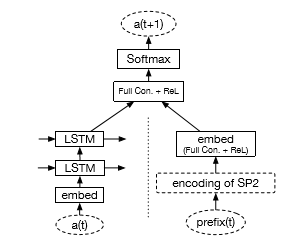
\includegraphics[height=.5\textwidth]{gfx/spice-winner-architecture.png}
    \caption{The neural network architecture of the winning submission at the SPiCE competition \cite{shibata2016bipartite}.}
    \label{fig:spice-winner-architecture}
\end{figure}

SP-$k$ languages are used to describe certain long-term dependencies through forbidding subsequences. If $\langle a,b \rangle$ is forbidden, then no $b$ may ever occur after $a$. A deterministic finite automaton (DFA) can also be used to characterize SP-$k$ languages, if its states encode the subsequences of size $k-1$  present in the previous prefixes \cite{heinz2010estimatingSP}. \autoref{tab:sp2-encoding} illustrates this encoding with a small example.

\begin{table}
    \centering
    \begin{tabular}{cclccccc}
        \hline
          &      &              & \multicolumn{5}{c}{SP-2 vector}\\
        t & a(t) & prefix(a(t)) & [a & b & c & d & e]\\
        \hline
        0 & a    & a            & [1 & 0 & 0 & 0 & 0]\\
        1 & d    & ad           & [1 & 0 & 0 & 1 & 0]\\
        2 & a    & ada          & [1 & 0 & 0 & 1 & 0]\\
        3 & c    & adac         & [1 & 0 & 1 & 1 & 0]\\
        4 & d    & adacd        & [1 & 0 & 1 & 1 & 0]\\
        \hline
    \end{tabular}
    \caption{Exemplary SP-2 encoded prefixes with $\sum=\{a,b,c,d,e\}$, abridged from Shibata et al.  \cite{shibata2016bipartite}. \textbf{TODO USE SEQUENCE NOTATION HERE}}
    \label{tab:sp2-encoding}
\end{table}